%
% lorenz.tex -- Lorenz-Modell
%
% - Herleitung aus den Gleichungen der Fluiddynamik
% - Dynamik aus numerischen Simulationen
%
% (c) 2018 Prof Dr Andreas Müller, Hochschule Rapperswil
%
\section{Lorenz-Modell}
Sowohl die Atmosphäre als auch die Ozeane werden durch die hydrodynamischen
Gleichungen beschrieben.
Es stellt sich damit die Frage, in welchem Masse sich daraus eine praktikable
Vorhersage sowohl von Wetter also auch des Klimas ableiten lässt.
In den Sechzigerjahren hat Edward Lorenz versucht, diese Frage mit einem
vereinfachten Modell zu beantworten.
Ziel dieses Abschnittes ist, das Lorenz-Modell aus den Gleichungen der
Fluiddynamik herzuleiten.

\subsection{Modellbeschreibung}
\begin{figure}
\centering
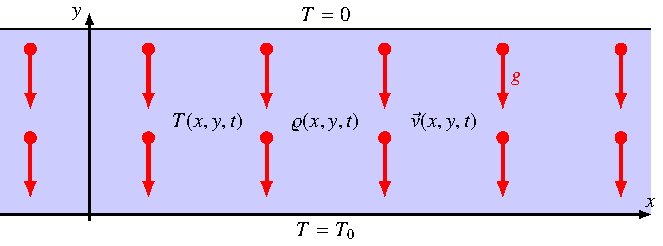
\includegraphics{chapters/1/lorenz-definition.pdf}
\caption{Definitionsgebiet für das Lorenz-Modell der Atmosphäre.
Gesucht sind Temperatur $T(x,y,t)$, Dichte $\varrho(x,y,t)$ und
Geschwindigkeit $\vec{v}(x,y,t)$ in einem Rechteckgebiet
$\mathbb R\times [0,\pi]$.
Die Temperatur ist an den Rändern vorgegeben, es gilt
$T(x,0,t)=T_0$ und $T(x,\pi,t)=0$.
Im Inneren Gebiet wird die Schwerkraft $g$ auf die Luft.
\label{skript:lorenzmodell definitionsgebiet}}
\end{figure}
Es soll ein dünner Schnitt durch die Atmosphäre modelliert werden.
Da Atmosphäre im Vergleich zur Krümmung der Erdoberfläche sehr dünn ist,
können wir sie als eben annehmen.
Wir verwenden die Koordinate $x$ parallel zur Erdoberfläche und $y$ als Höhe
(Abbildung~\ref{skript:lorenzmodell definitionsgebiet}).
Gesucht ist also die Temperatur $T(x,y,t)$ und die Dichte $\varrho(x,y,t)$
in Abhängigkeit von Position und Zeit sowie der Geschwindigkeitsvektor
\[
\vec v
=
\begin{pmatrix}v_x\\v_y\end{pmatrix}
=
\begin{pmatrix}v_x(x,y,t)\\v_y(x,y,t)\end{pmatrix}.
\]
Die Funktionen $T$, $\varrho$, $v_x$ und $v_y$ sind definiert in einem
Streifen.
Der Einfachheit halber wählen wir die Höhe des Streifens als $\pi$.
Wir können dies erreichen, indem wir die Längeneinheit geeignet wählen:
ist $h$ die ``Dicke'' der Atmosphäre\footnote{Die Konvektion in der Atmosphäre,
welche vom Lorenz-Modell vor allem beschrieben wird, findet im Wesentlichen
nur im untersten Teil der Atmosphäre, der sogenannten Troposphäre statt.
Die Troposphäre zeichnet sich aus durch mehr oder weniger lineare
Temperaturabnahme bis zur Höhe der sogenannten Tropopause in etwa
10km Höhe.
Wir können also die Höhe der Tropopause als $h$ verwenden.}, wählen wir
$h/\pi$ als Längeneinheit.
Das Definitionsgebiet für die Funktionen ist daher $R=\mathbb R\times [0,\pi]$.

Die Temperatur der Atmosphäre an der Erdoberfläche wird im wesentlichen von
der Temperatur des Bodens bestimmt, der von der einfallenden Strahlung
ergewärmt wird, es soll also $T(x,0,t)=T_0$ gelten.
Am oberen Rand des Schnittes schliesst die sehr dünne Hochatmosphäre an,
die im Wesentlichen in einem Strahlungsgleichgewicht mit der Umgebung steht.
Da wir die Dichte im wesentlichen als konstant ansehen wollen und damit
den Einfluss der Temperatur auf die Dichte nicht exakt modellieren wollen,
sind wir nicht gezwungen, eine bestimmte Temperaturskala zu verwenden.
Wir können daher willkürlich die Temperatur am oberen Rand als
$T(x,\pi,t)=0$ festlegen.

Auf das Medium im Streifen wirkt natürlich die Erdbeschleunigung,
die wir ebenfalls als konstant annehmen dürfen, da die Dicke der 
Atmosphäre im Vergleich zum Erdradius sehr klein ist.

\subsubsection{Stabile Atmosphäre}
\begin{figure}
\centering
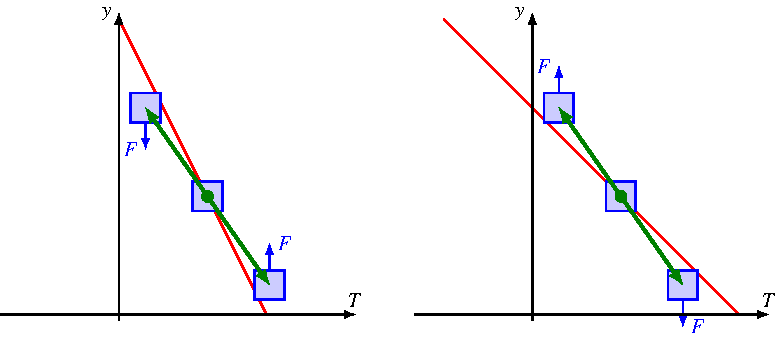
\includegraphics{chapters/1/lorenz-stabil.pdf}
\caption{Stabilität der Atmosphäre: bewegt sich ein Luftpaket in der
Atmosphäre nach oben oder unten, expandiert oder kontrahiert es und
verändert seine Temperatur adiabatisch (grün).
Ist diese Temperaturänderung grösser als der aktuelle Temperaturgradient
(links),
ändert sich die Dichte der Luft weniger stark als die der Umgebungsluft,
die Bewegung wird gestoppt, die Atmosphäre ist im Gleichgewicht.
Andernfalls wird die Bewegung beschleunigt, die Atmosphäre ist instabil
(rechts).
\label{skript:stabilitaet der atmosphaere}}
\end{figure}
Die Temperatur muss im Gebiet von unten nach oben abnehmen.
Aber auch der Druck muss mit zunehmender Höhe abnehmen. 
Wenn ein Luftpaket aufsteigt, wird es wegen des geringer werdenden
Druckes expandieren und damit adiabatisch abkühlen.
Wenn die Temperatur der umgebenden Luft schneller abnimmt als die
adiabatische Abkühlung, dann ist das Luftpaket in seiner neuen Höhe
wärmer und damit leichter als die Umgebung, es wird weiter ansteigen
(Abbildung~\ref{skript:stabilitaet der atmosphaere}).
Wenn die Temperatur der umgebenden Luft langsamer abnimmt als die
adiabatische Abkühlung, dann ist das Luftpaket in der neuen Höhe 
kälter und damit Dichter als die Umgebung, es wird wieder absinken.
Solange der Temperaturunterschied nicht zu gross ist, wird sich also ein
Zustand einstellen, in dem die Luft in Ruhe bleibt, der Wärmetransport
erfolgt ausschliesslich durch Wärmeleitung.

\subsubsection{Instabilität}
Bei genügend grosser Temperaturdifferenz wird die Atmosphäre jedoch
instabil, der Wärmetransport wird zusätzlich von Konvektion übernommen.
Die entstehenden Konvektionszellen können wegen der Translationssymmetrie
entlang der $x$-Achse an einer beliebigen Stelle entstehen, es gibt also
unendlich viele Lösungen, von denen eine gewählt werden muss.
In der Realität würden kleine Temperaturfluktionen dies unterstützen,
kleine Unterschiede in den Anfangsbedingungen führen also zu völlig
verschiedenen Strömungen.
% Abbildung?
Diese sensitive Abhängigkeit der Lösung von Anfangsbedingungen wird
oft als ein Kennzeichen von Chaos angesehen.

Im folgenden sollen zunächst die Gleichungen der Fluiddynamik auf die
vorliegende Situation spezialisiert werden.
Mit Hilfe eines geeigneten Ansatzes soll dann die partielle
Differentialgleichung weiter auf ein System von gewöhnlichen 
Differentialgleichungen reduziert werden.
In numerischen Simulationen soll schliesslich gezeigt werden, dass die 
Lorenz-Gleichungen tatsächlich chaotische Lösungen haben.

\subsubsection{Kontinuitätsgleichung}
\subsubsection{Bewegungsgleichung}

\subsection{Grundgleichungen}

\subsection{Umwandlung in ein gewöhnliches Differentialgleichungssystem}

